\begin{frame}
\frametitle{NEXT White (NEW)} 

 \begin{center}
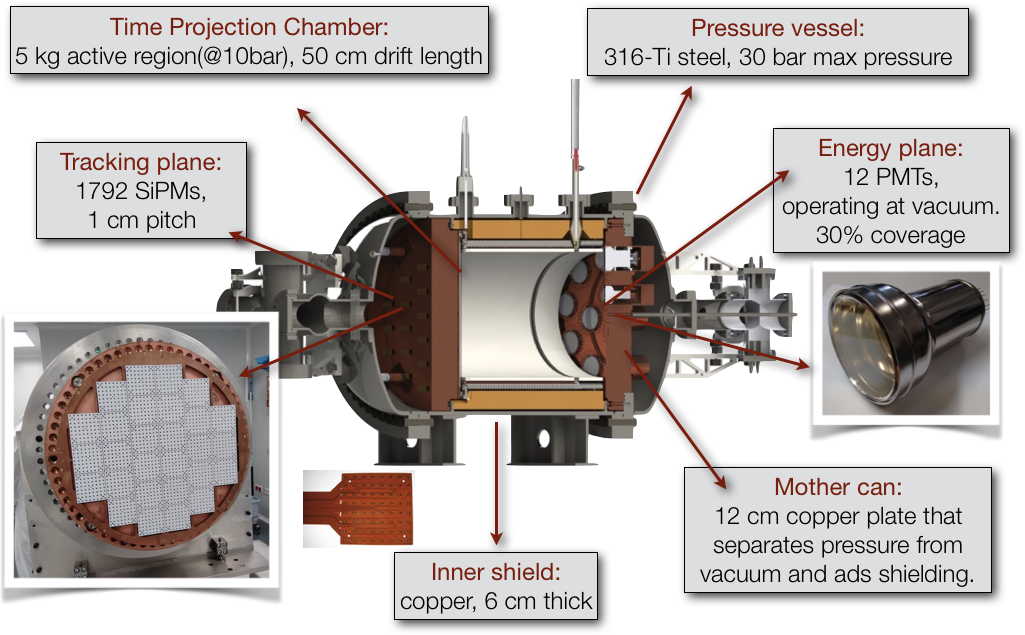
\includegraphics[width=0.85\textwidth]{moriond/next-white-drawing.png}
\end{center}
\end{frame}

\begin{frame}
 \begin{center}
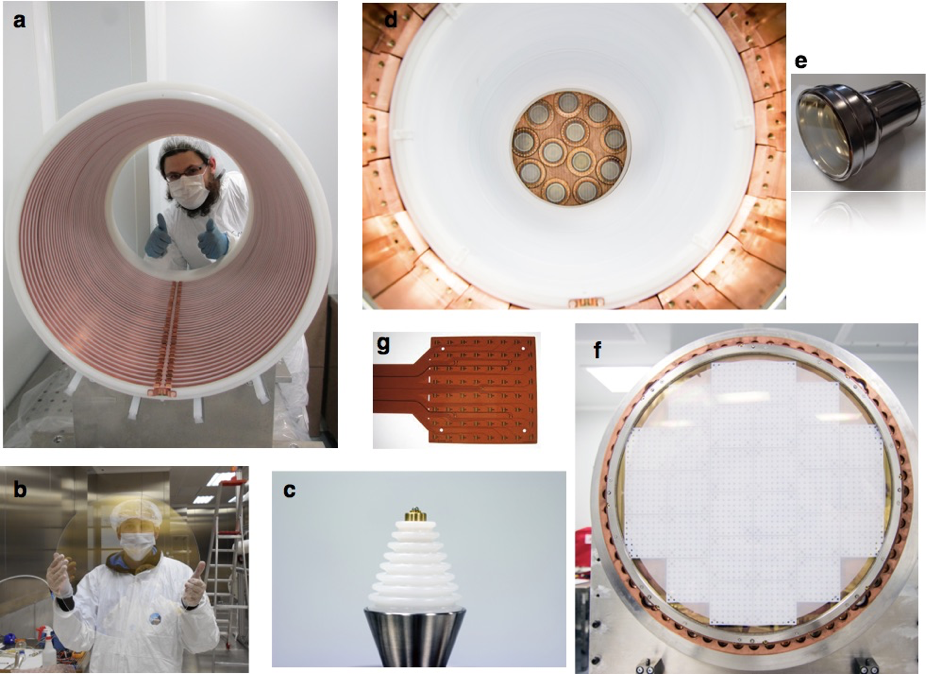
\includegraphics[width=0.85\textwidth]{moriond/next-parts.png}
\end{center}
\end{frame}

\begin{frame}
 \begin{center}
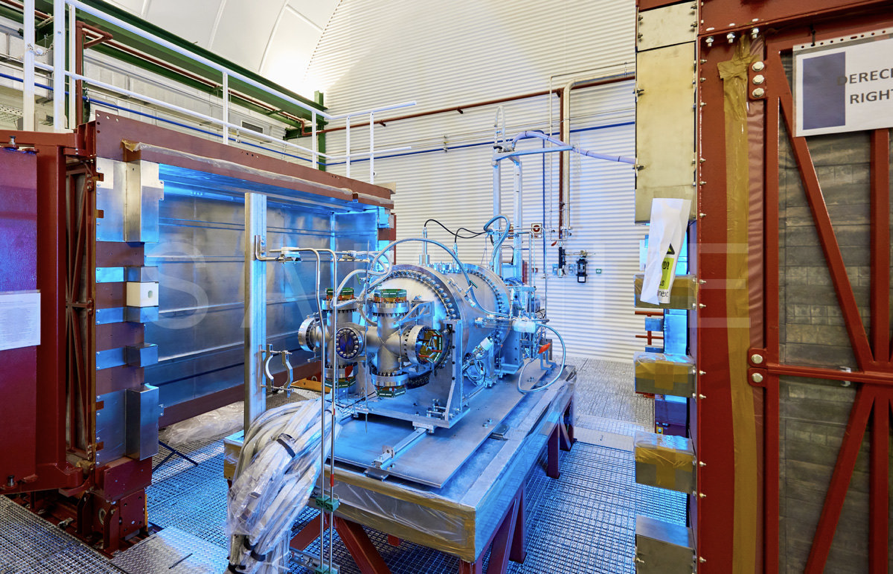
\includegraphics[width=0.85\textwidth]{moriond/next-white.png}
\end{center}
\end{frame}

\begin{frame}
\frametitle{Goals of NEW} 
\begin{itemize}
\item Demonstrate technology is robust. 
\item Demonstrate energy resolution and topological signature. 
\item Measure backgrounds to establish a reliable background model (and to improve it as needed). 
\end{itemize}
\end{frame}

\begin{frame}
\frametitle{Operation of NEW} 
 \begin{center}
 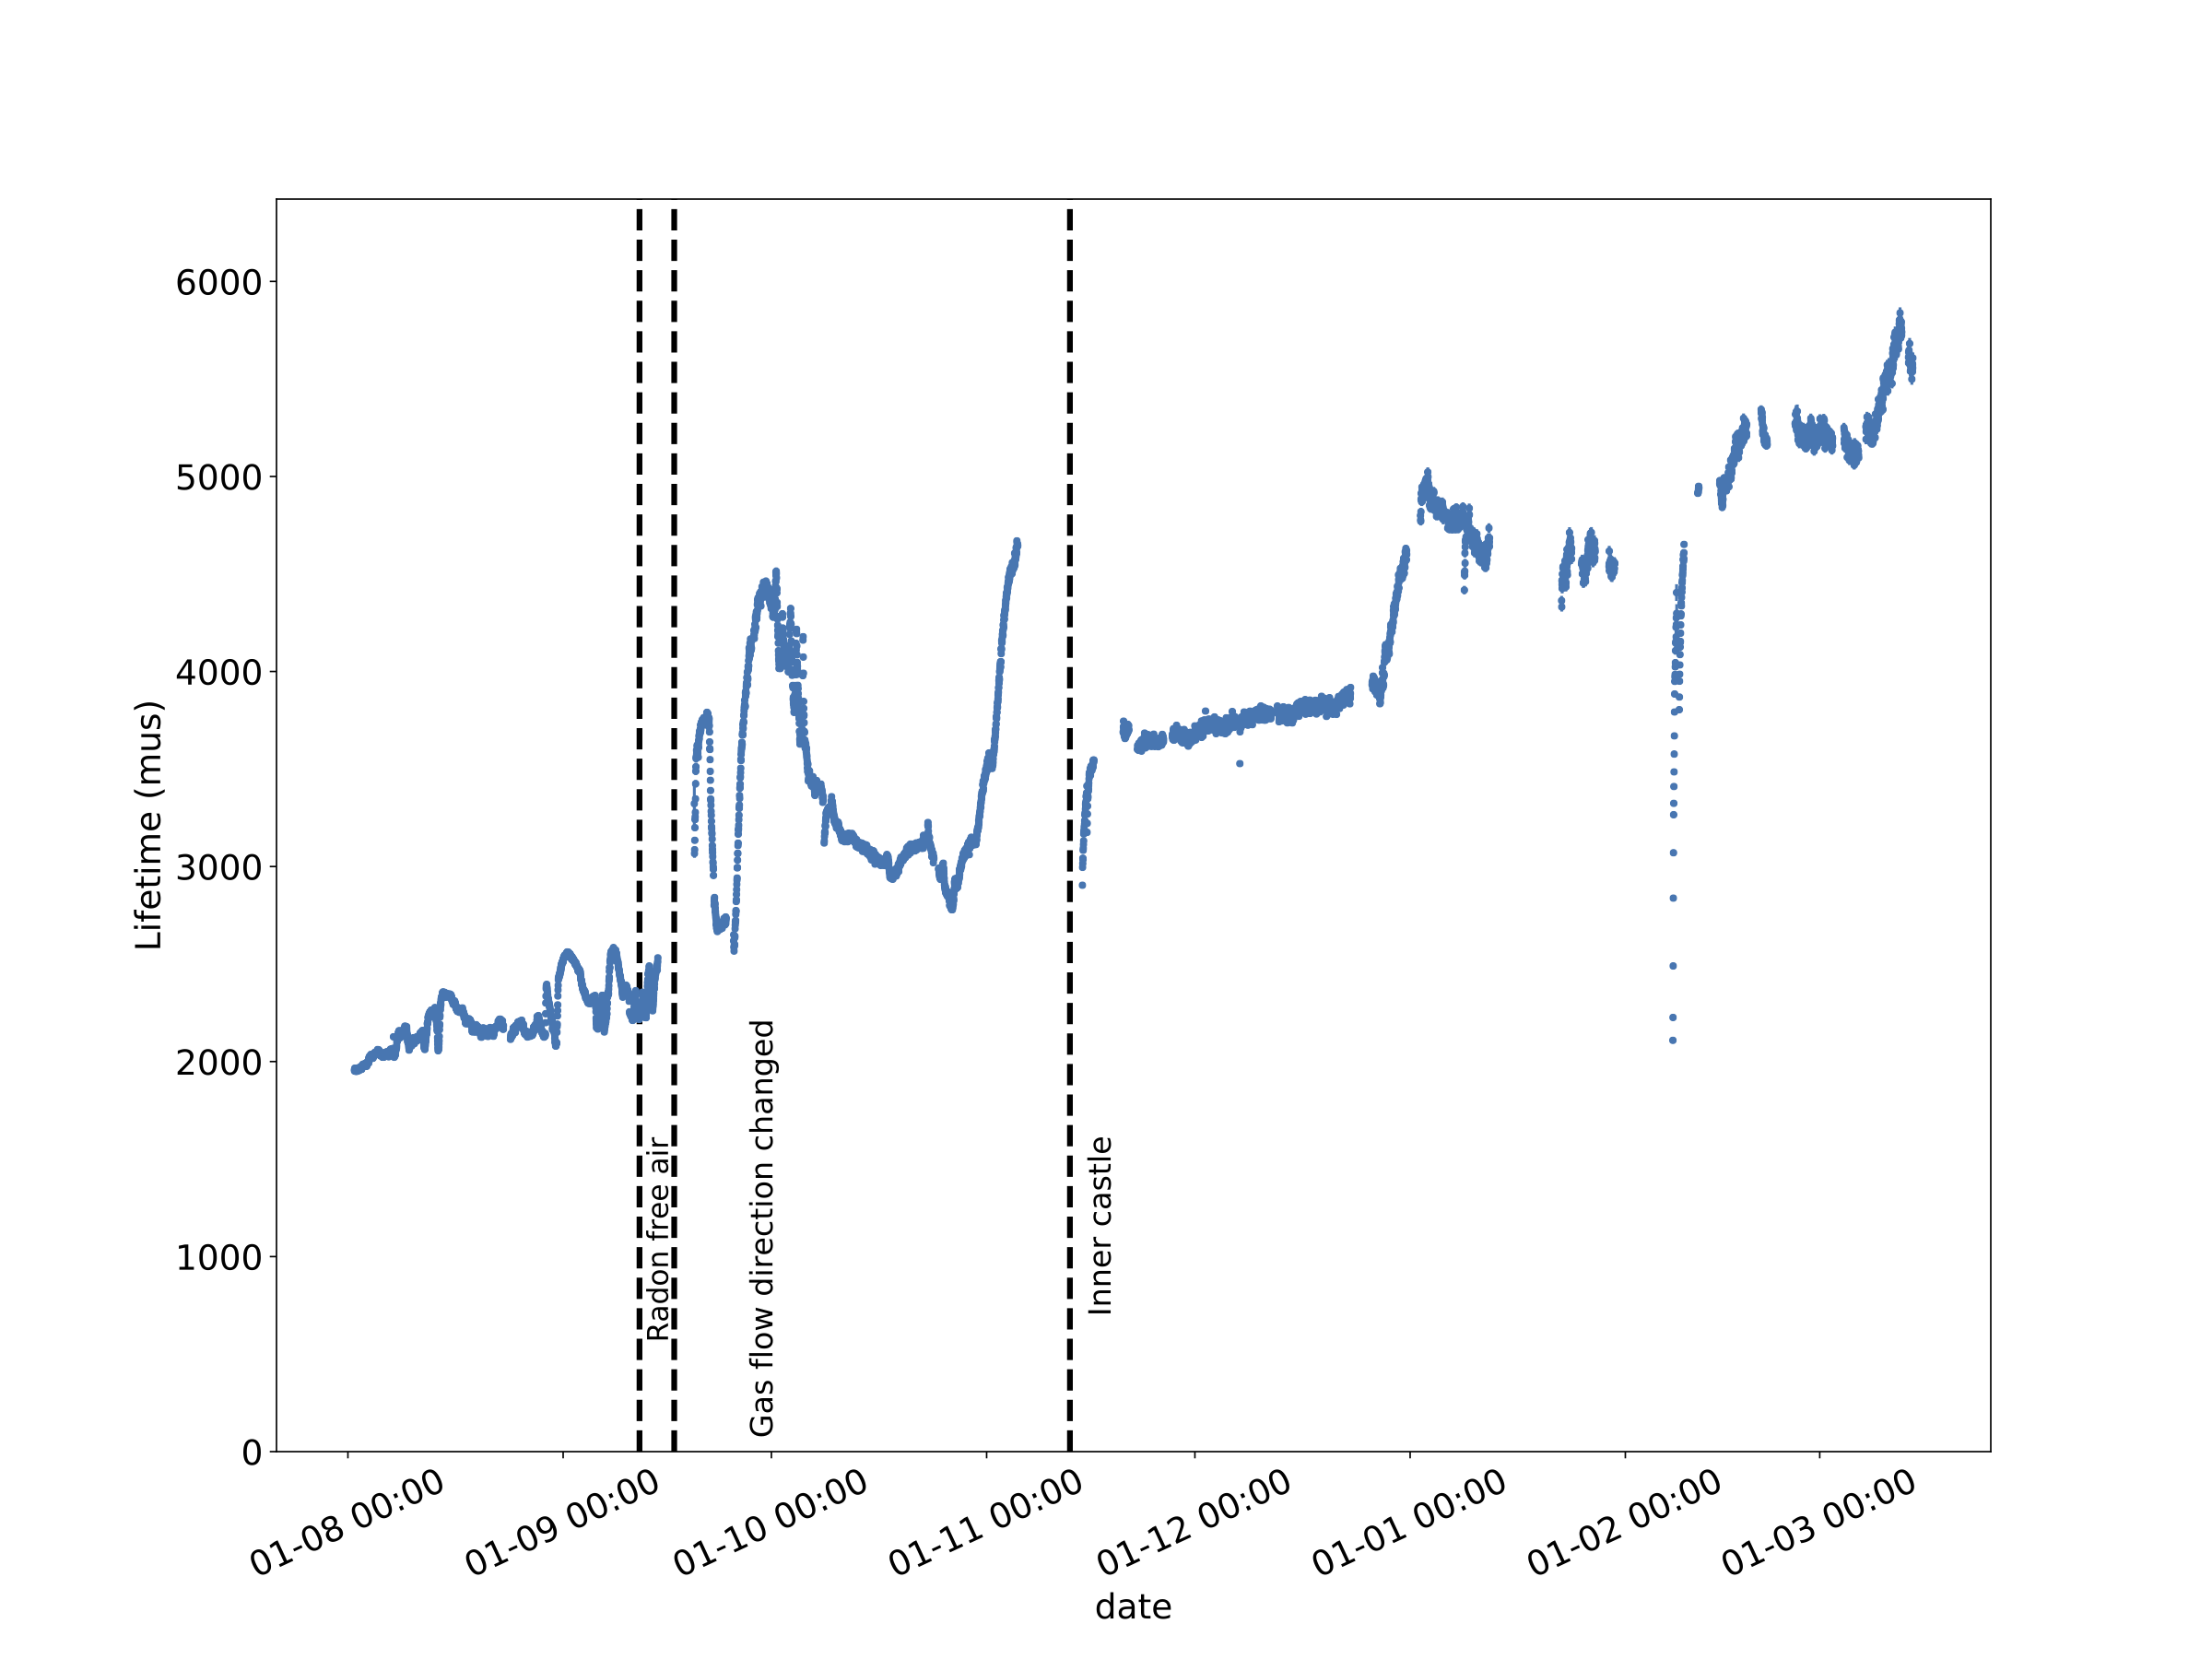
\includegraphics[width=0.65\textwidth]{moriond/lifetime_evolution.png}
\end{center}
\begin{itemize}
\item Taking data since 2016. Very stable operation since 2017.
\item Less than 1 gram of gas lost per year. 
\item Very high lifetime, measured on a daily basis with Krypton calibrations. 
\end{itemize}
\end{frame}

\begin{frame}
 \frametitle{NEW energy resolution} 
 \begin{center}
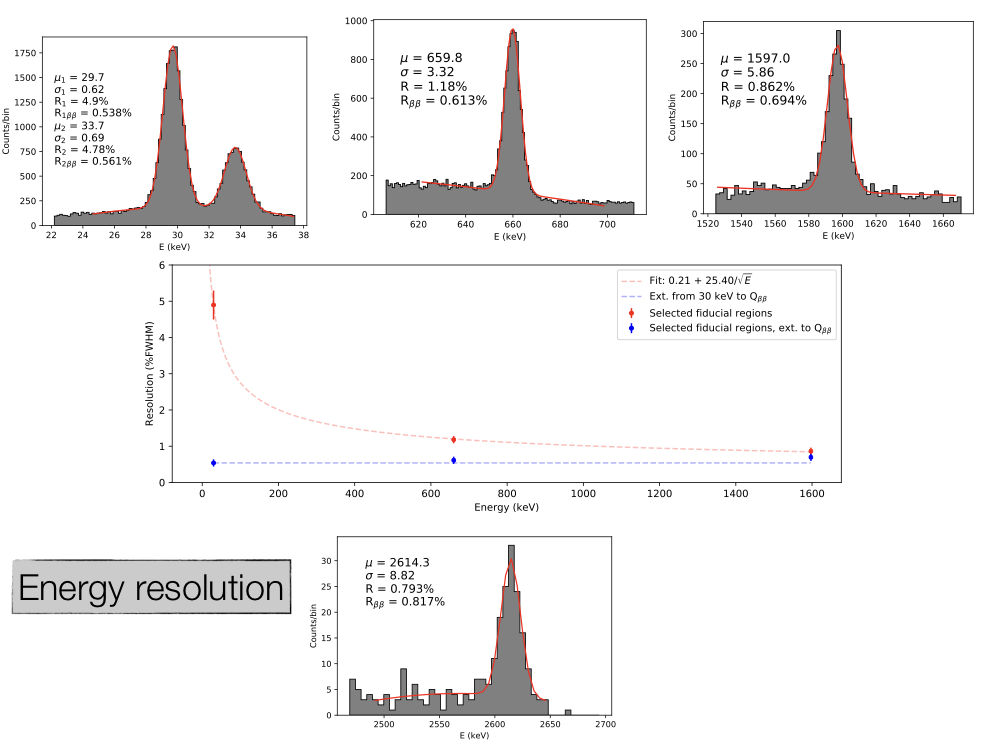
\includegraphics[width=0.85\textwidth]{moriond/new_energy_res.png}
\end{center}
\end{frame}

\begin{frame}
 \frametitle{NEW topological signature} 
 \begin{center}
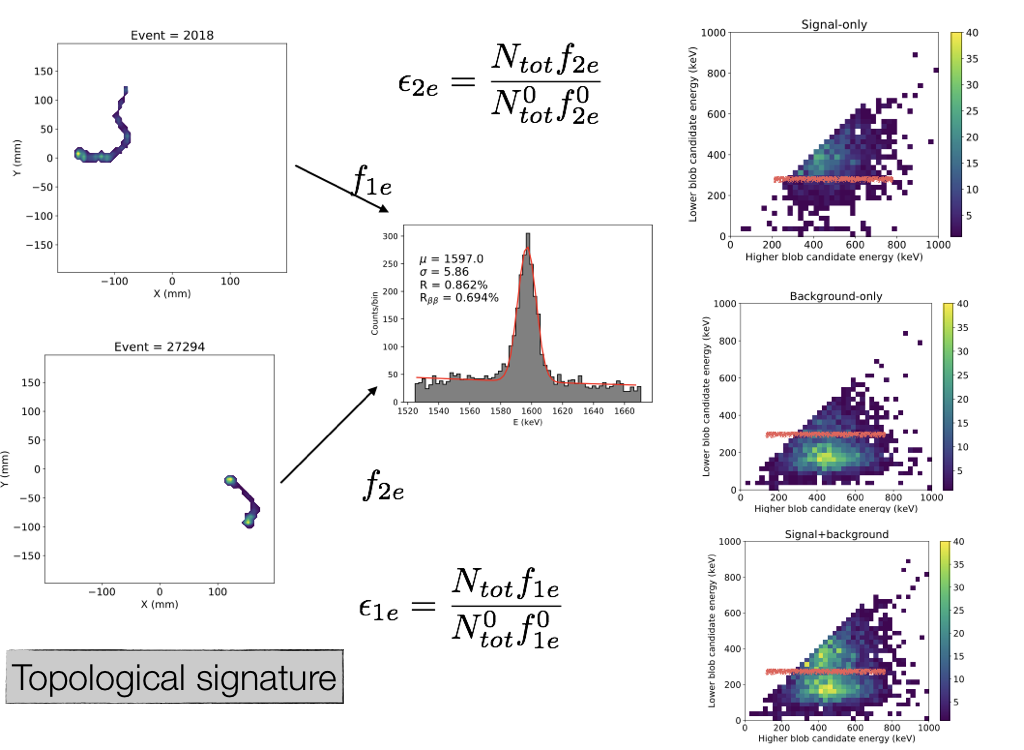
\includegraphics[width=0.85\textwidth]{moriond/new_topo_doublescape.png}
\end{center}
\end{frame}

\begin{frame}
 \begin{center}
 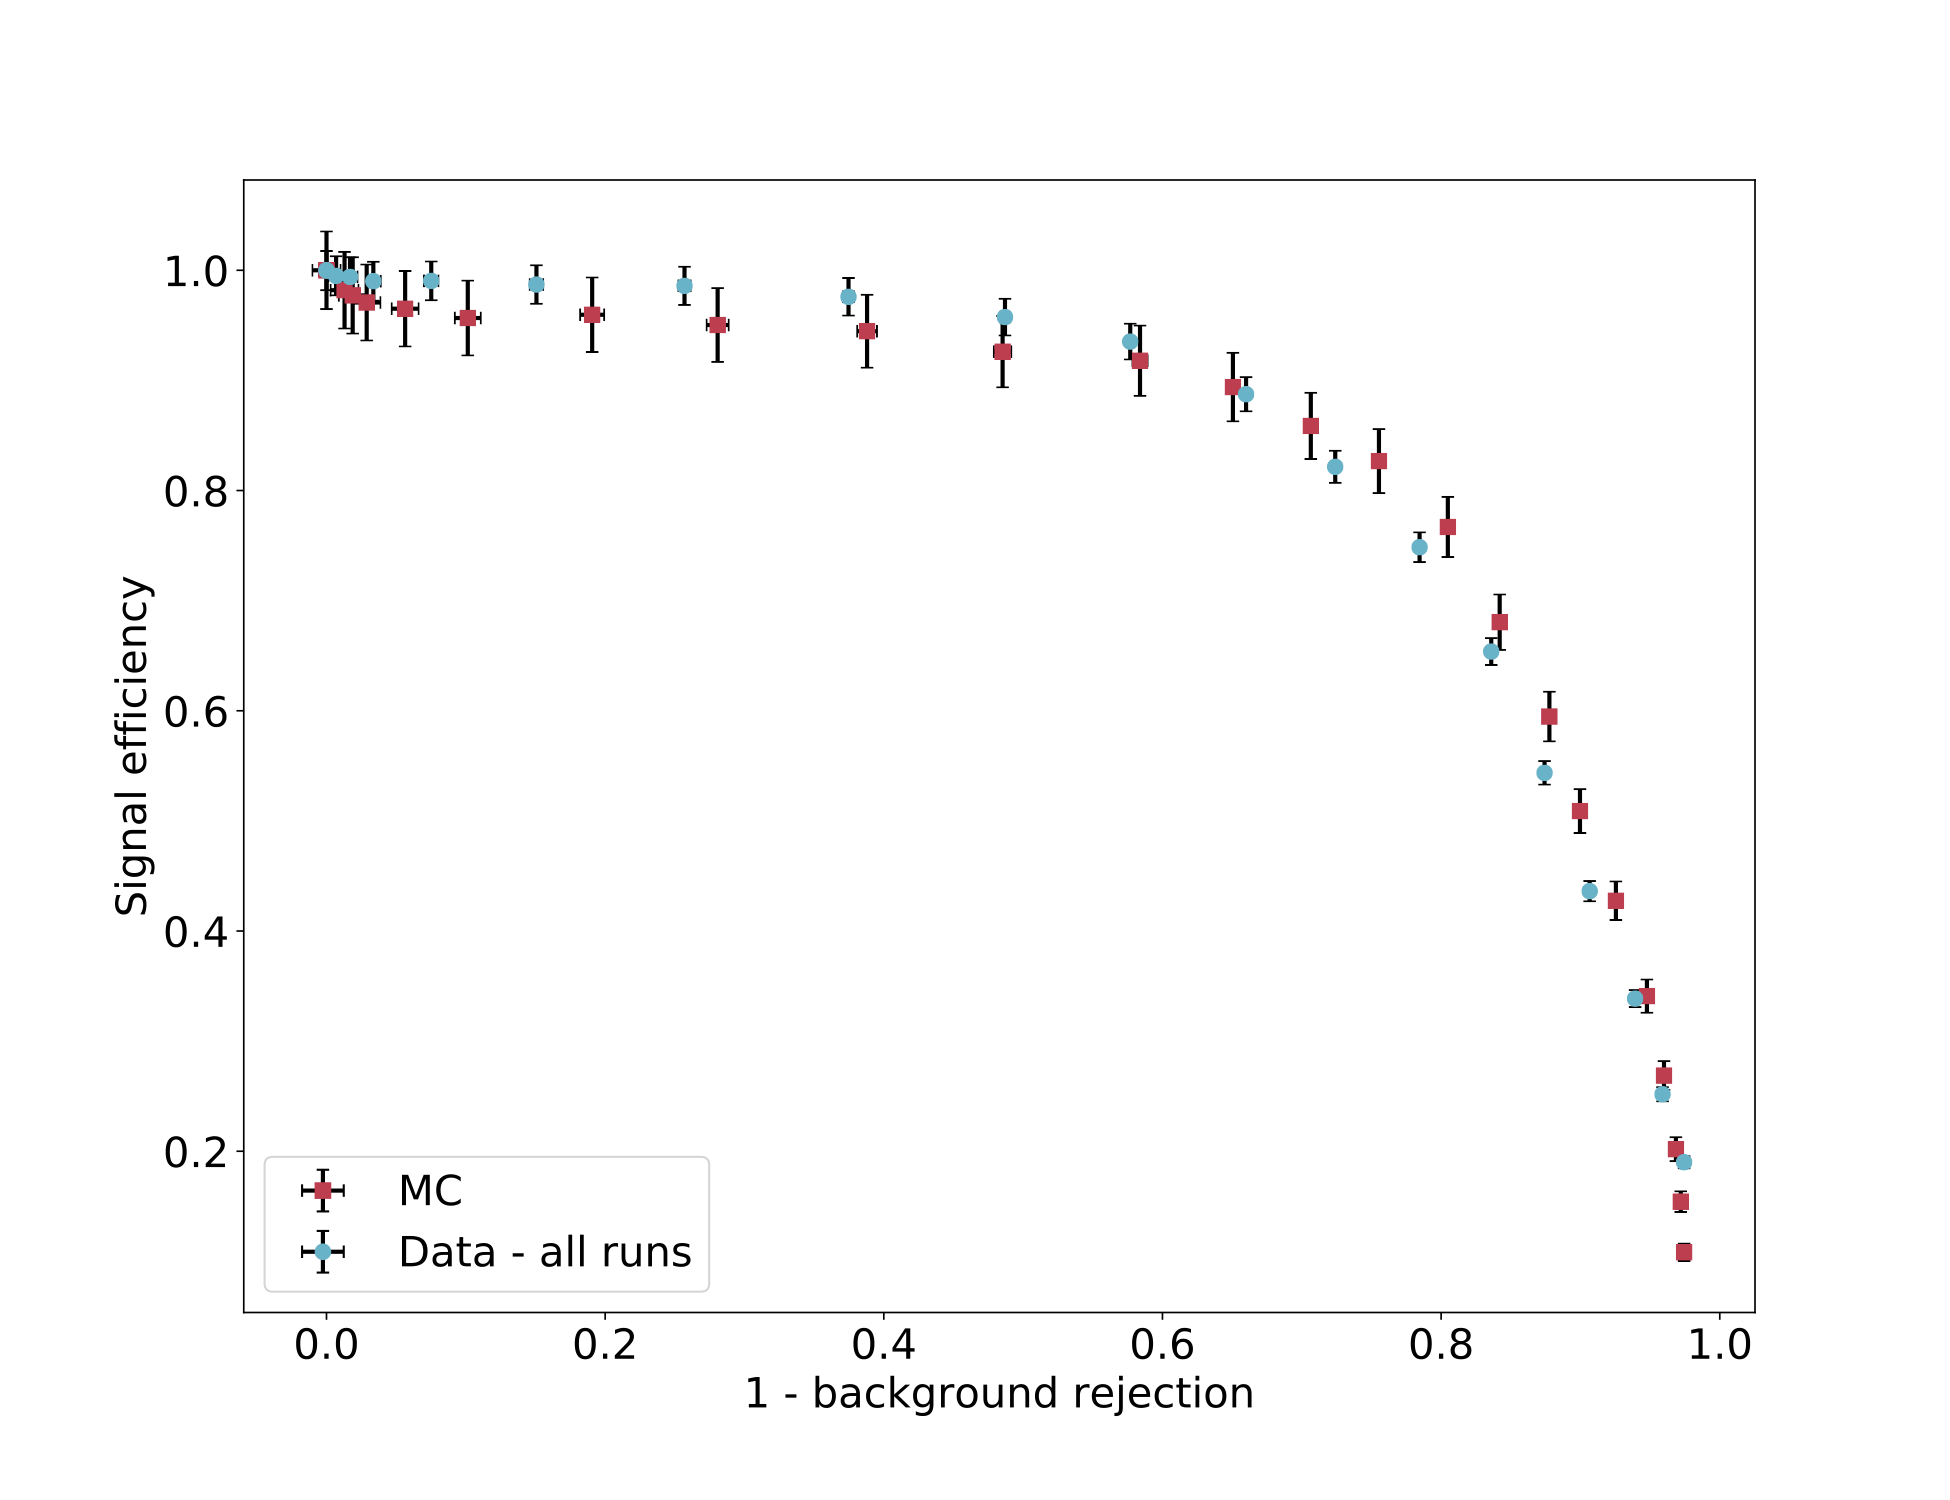
\includegraphics[width=0.45\textwidth]{moriond/new_topo_data_mc.png}
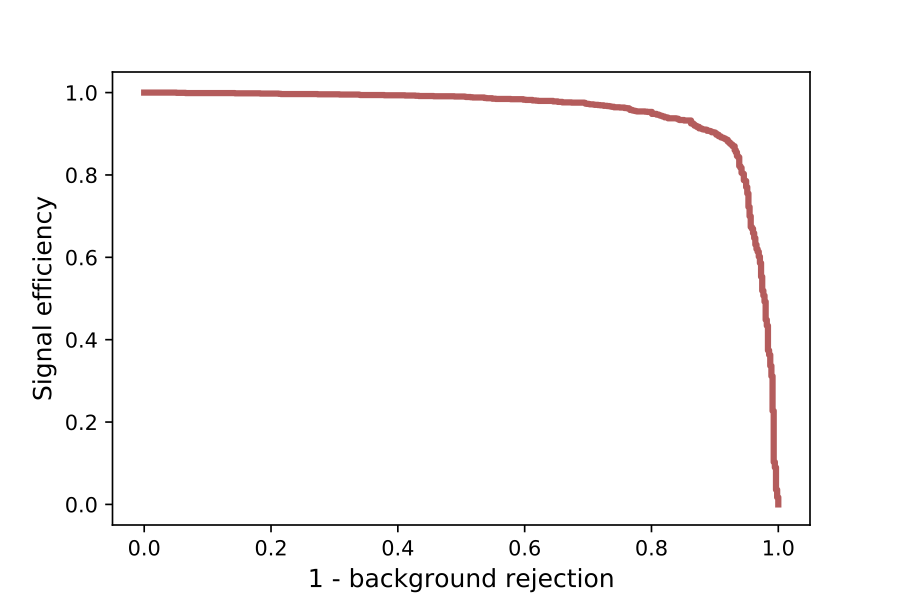
\includegraphics[width=0.50\textwidth]{moriond/eff_vs_bkg_dnn.png}
\end{center}

\begin{itemize}
\item {\bf Blob analysis}, in \TL\ double escape peak shows good agreement data/MC. 
\item {\bf DNN analysis}, optimizes separation signal/background. Shown MC prediction: 90 \% signal efficiency 10\% background contamination. 
\end{itemize}
\end{frame}





